%#!platex main

\newcommand{\First}{{\sf FIRST}}
\newcommand{\Follow}{{\sf FOLLOW}}
\newcommand{\Director}{{\sf DIRECTOR}}

\chapter{構文解析}

\section{構文解析の手法}

構文解析部は、字句解析部から出力されたトークン列を読み込み、原始プログラ
ミング言語の文法に適合しているか解析し、適合している場合はトークンを意味
のまとまりを反映した入れ子構造にグループ化したものを出力する。

ところで、原始プログラム言語の文法が(トークンを終端記号とするような)文
脈自由文法で記述されている、としよう。すると、構文解析部の出力は、トーク
ン列を結果とするような解析木に他ならない。つまり構文解析とは、文脈自由文
法をもとにトークン列を導出し、解析木を構成する作業そのものである。ただし、
考えておかなければならないことがいくつかある。

1つ目は、構文解析の計算量(計算時間)である。どんな文脈自由文法でも、それ
に基づいた構文解析ルーチンは作れるのだが、一般には、長さ$n$のトークン列の
構文解析に$O(n^3)$の時間が必要となってしまうのである。対象とするトークン
列が原始プログラムであり、サイズが大きくなりうることを考えると、これでは
計算時間がかかりすぎると言える。そこで、コンパイラの構文解析では、文法に
制限を加え、$O(n)$程度の時間で構文解析を可能にするのが普通である。

2つ目は、構文解析プログラムの設計の方針である。対象とするトークン列の長さ
が事前には分からず、かつ大きくなりうるため、トークン列をあらかじめ全部読
み込んでから解析を行う、というプログラム設計は好ましくない。そこで、この
講義では、字句解析部から構文解析部に1トークンずつ渡しながら解析を行う、と
いう手法をとる。このため、見かけ上、文脈自由文法での導出とは異なるアルゴ
リズムになっている。

構文解析の手法には、解析木を作る方向によって大きく2種類に分けられる。根か
ら葉に向けて作る手法を{\bfseries 下向き構文解析}(top-down parsing)、葉
から根に向けて作る手法を{\bfseries 上向き構文解析}(bottom-up parsing)と
いう。下向き構文解析のほうが手法としては易しく、手作業で構文解析ルーチン
を作れるが、文法に対する制限は大きい。ただし、それでもほとんどのプログラ
ミング言語の構文解析には十分である。そこで、この講義では、下向き構文解析
に絞って解説する。

\section{予測型構文解析}

次の文脈自由文法を例にとり、下向き構文解析を説明しよう。この文法はPascal
というプログラミング言語の型宣言の一部である。
\begin{equation}
\begin{split}
 type & \rightarrow simple \mid \text{\^{}}\ id
 \mid \text{{\sffamily array}}\ \text{{\sffamily [}}\ simple\ \text{{\sffamily ]}}\ \text{{\sffamily of}}\ type \\
 simple & \rightarrow \text{{\sffamily integer}} \mid \text{{\sffamily
 char}} \mid \text{{\sffamily num}}\ \text{{\sffamily dotdot}}\ \text{{\sffamily num}}
\end{split}\label{151415_10Apr06}
\end{equation}

この文法でトークン列\icode{array [ num dotdot num ] of integer}の解析木を
作る過程を図\ref{154017_30Mar06}に示す。

\begin{figure}
 \begin{center}
  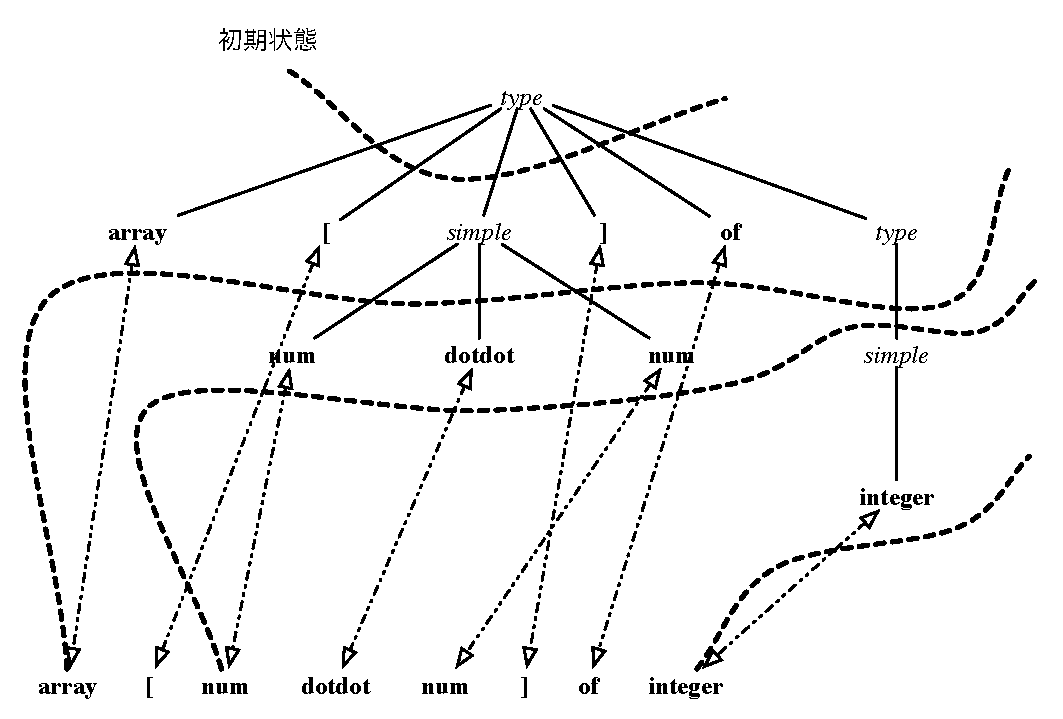
\includegraphics[width=12cm]{figure/making_parse_tree.pdf}
 \end{center}
 \caption{解析木の構成過程}
 \label{154017_30Mar06}
\end{figure}

最初、節点は開始記号$type$だけであり、制御はこの節点にある。字句解析部か
ら先頭のトークン{\sf array}が渡されると、$type$を左辺に持つ生成規則のうち、
{\sf array}を先頭とする記号列を生成する可能性のある規則を探す。この場合は
$type \rightarrow {\sf array [}\ simple\ {\sf ] of}\ type$のみが該当する。
そこで、この規則の右辺の各記号を、順に$type$の子節点とし、制御を子節点の
先頭、すなわち{\sf array}とラベル付けされた節点に移す。ラベル{\sf array}
は終端記号なので、現在のトークン{\sf array}と照合する。照合に成功すれば、
次のトークンを読み込み、また、現在の解析木で深さ優先順に次の節点、つまり
{\sf [}とラベル付けされた節点に制御を移して、同様の処理を続ける。

この処理から分かるように、上の文法では、トークン列を左から右に1回走査する
だけで下向きに解析木を構成することができる。このような(下向き)構文解析
手法を特に{\bfseries 予測型構文解析}(predictive parsing)という。「予測」
という言葉は、次に作ろうとしている節が非終端記号の場合、現在のトークン1つ
だけで、どの生成規則を適用して導出を進めればよいか、予測できるという事実
に由来している。

後述するように、予測型構文解析ルーチンは非常に簡単に実装できる。しかし、
どんな文法でも予測型構文解析が行えるわけではない。かなり制限された形の文
法でしか、この解析手法は使えない。それでも、実用上は、予測型構文解析が行
える程度の文法で充分な場合がかなり多い。

文法$G$について予測型構文解析が可能であるためには、$G$が次のような制限を
満たしていなければならない。
\begin{enumerate}
 \item $G$は曖昧でなく、かつ左再帰ではない。
 \item 生成規則$A \rightarrow \alpha_1 \mid \alpha_2 \mid \cdots \mid
       \alpha_n $について、現在の入力記号$a$のみからどの生成規則で$A$を書
       き換えればよいか、一意に決定できなければならない。
\end{enumerate}

以下で対象とするのは、曖昧でなく、左再帰ではない文法とする。もし構文解析
を行いたい文法が曖昧であったり左再帰であったりする場合は、
\ref{121131_31Mar06}節や\ref{121145_31Mar06}節の手法を用いて、曖昧でなく
左再帰でない文法に変形しておかなければならない。

\section{LL(1)文法}
\label{160007_10Apr06}

予測型構文解析の可能な文法として、{\bfseries LL(1)文法}(LL(1) grammar)
という文法を紹介する。多くのプログラミング言語の文法はLL(1)文法に収まって
いることが知られている。

\subsection{\First と\Follow}

まず\First と\Follow という2つの終端記号集合を導入しておこう。

任意の記号列$\alpha$に対し、$\alpha$から導出される記号列の中で先頭に現れ
る終端記号の集合を$\First(\alpha)$という。ただし$S
\stackrel{*}{\Rightarrow} \epsilon$の場合は$\epsilon$も
$\First(\alpha)$に含める。

非終端記号$A$に対し、文形式の中で、$A$のすぐ後ろに現れる可能性のある終端
記号の集合を$\Follow(A)$とする。$A$が文形式の一番後ろになることが
ある場合には、記号列の末尾を表す特殊な終端記号$\$$を$\Follow(A)$
に含める。

\begin{example}
 \label{ex:first_follow}
 次の(曖昧でなく左再帰でない)文法を考える。
 \begin{align*}
  E & \rightarrow TE' \\
  E' & \rightarrow + TE' \mid \epsilon \\
  T & \rightarrow FT' \\
  T' & \rightarrow * FT' \mid \epsilon \\
  F & \rightarrow (E) \mid \mathbf{id}
 \end{align*}
 この文法に対し、\First を求めると次のようになる。
 \begin{align*}
  & \First(E) = \First(T) = \First(F) = \{(, \mathbf{id}\} \\
  & \First(E') = \{+, \epsilon\} \\
  & \First(T') = \{*, \epsilon\} \\
  & \First(TE') = \First(T) = \{(, {\bf id}\} \\
  & \First(\epsilon) = \{\epsilon\} \\
  & \First(+TE') = \{+\} \\
  & \First(FT') = \First(F) = \{(, {\bf id}\} \\
  & \First(*FT') = \{*\} \\
  & \First((E)) = \{(\} \\
  & \First({\bf id}) = \{{\bf id}\}
 \end{align*}
 また\Follow を求めると次のようになる。
 \begin{align*}
  & \Follow(E) = \Follow(E') = \{), \$\} \\
  & \Follow(T) = \Follow(T') = \{+, ), \$\} \\
  & \Follow(F) = \{+, *, ), \$\}
 \end{align*}
 $\Box$
\end{example}

\subsection{\First の計算方法}

\begin{enumerate}
 \item 終端記号$a$について$\First(a) = \{a\}$
 \item $\epsilon$について$\First(\epsilon) = \{\epsilon\}$ 
 \item 生成規則$X \rightarrow a\alpha$について、$a$を$\First(X)$
       に加える。
 \item 生成規則$X \rightarrow \epsilon$について、$\epsilon$を
       $\First(X)$に加える。
 \item 生成規則$X \rightarrow Y_1Y_2\cdots Y_n$について
       \begin{itemize}
	\item $Y_1$が$\epsilon$を導出しないならば$\First(Y_1)$を
	      $\First(X)$に加える
	\item $Y_1 \stackrel{*}{\Rightarrow} \epsilon$であれば、
	      $\First(Y_1) - \{\epsilon\}$を$\First(X)$に加える。さらに
	      $Y_2$が$\epsilon$を導出しないならば、$\First(Y_2)$を
	      $\First(X)$に加え、$Y_2 \stackrel{*}{\Rightarrow}
	      \epsilon$ならば$\First(Y_2) - \{\epsilon\}$を
	      $\First(X)$に加える。(以下同様)
	\item $Y_1Y_2\cdots Y_n \stackrel{*}{\Rightarrow} \epsilon$ならば、
	      $\epsilon$を$\First(X)$に加える
	      \label{170823_7Jun05}
       \end{itemize}
 \item $\First(X_1X_2\cdots X_n)$は\ref{170823_7Jun05}と同様に計算
\end{enumerate}

規則\ref{170823_7Jun05}がやや分かりにくいかもしれない。例えば、生成規則$X \rightarrow
Y_1Y_2$について、ある終端記号$x$が$\First(X)$に含まれるのは、次のいずれ
かの場合に限られる。
\begin{enumerate}
 \item $x \in \First(Y_1)$
 \item $Y_1 \stackrel{*}{\Rightarrow} \epsilon$かつ$x \in \First(Y_2)$
\end{enumerate}
つまり$Y_1$から終端記号が何も生成されない可能性があるならば、
$\First(Y_2)$の要素も$\First(X)$に含まれる、ということである。規則
\ref{170823_7Jun05}はこれを一般的にしたものである。

\subsection{\Follow の計算方法}

\begin{enumerate}
 \item $\Follow(S)$に$\$$を加える。
 \item どの\Follow にも記号が追加されなくなるまで、以下を繰り返す。
       \begin{itemize}
	\item $A \rightarrow \alpha B\beta$について、$\First(\beta)
	      - \{\epsilon\}$を$\Follow(B)$に加える。
	\item $A \rightarrow \alpha B\beta$、かつ$\First(\beta)$
	      が$\epsilon$を含んでいるとき、$\Follow(A)$を
	      $\Follow(B)$に加える。
	\item $A \rightarrow \alpha B$のとき、$\Follow(A)$を
	      $\Follow(B)$に加える。
       \end{itemize}
\end{enumerate}

やや分かりにくいアルゴリズムなので、少し整理してみよう。
$\Follow()$の値が変化するのは、次の3通りの場合しかない。
\begin{itemize}
 \item 開始記号$S$について、無条件に$\$$が加えられる。
 \item $A \rightarrow \alpha B \beta$の形の規則について、$\First(\beta)$
       が$\Follow(B)$に加えられる。($\beta$から導出される記号列の先頭の
       文字は$B$の直後に現れるから)
 \item $A \rightarrow \alpha B$、もしくは$A \rightarrow \alpha B \beta$
       で$\beta$から$\epsilon$が導出される($\beta$が消えてしまう)場合
       について、$\Follow(A)$が$\Follow(B)$に加えられる。($A$の直後に現れ
       る文字は$B$の直後にも現れるから)
\end{itemize}
そこで、生成規則を見ながら、値が伝搬していく様子を有向グラフにしてみる。
例えば$E \rightarrow TE'$から$\First(E') - \{\epsilon\}$が$\Follow(T)$
に伝搬することが分かるので、$\First(E')$から$\Follow(T)$へ有向枝を加える。
このとき、$\First(E')$から$\{\epsilon\}$を引かなければならないので、枝を
破線にしておく。また$E' \rightarrow +TE' \mid \epsilon$より$E'
\Rightarrow \epsilon$であるので、$\Follow(E')$が$\Follow(T)$に伝搬するこ
とが分かる。そこで、$\Follow(E')$から$\Follow(T)$へ有向枝を加える。

このようにすべての値の伝搬に対して有向枝を加えると、図
\ref{134551_20Jul07}のようなグラフが得られる。このグラフを用いて
$\Follow$を計算することができる。つまり、有向枝$X \rightarrow Y$がある場
合は$X$の要素をすべて$Y$に加える。また$X …> Y$がある場合は$X$の要素のう
ち$\epsilon$以外をすべて$Y$に加える。図\ref{134551_20Jul07}を基に
$\Follow$を計算すると、例\ref{ex:first_follow}に示した通りになることを確
かめよ。
\begin{figure}
 \begin{center}
  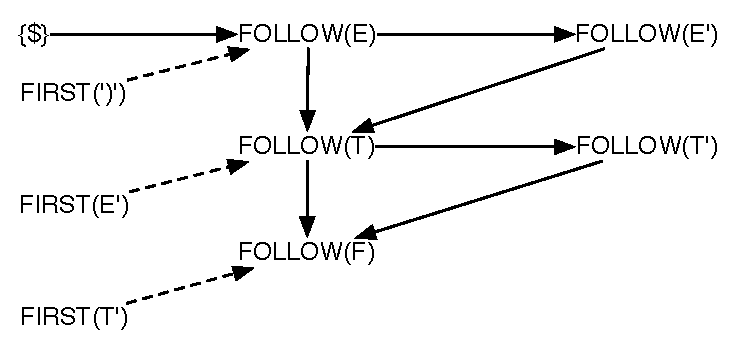
\includegraphics[scale=0.7]{figure/2008040801.pdf}
 \end{center}
 \caption{$\Follow$の値の伝搬を表すグラフ}
 \label{134551_20Jul07}
\end{figure}

\subsection{LL(1)文法}

\subsubsection{\Director}

上で述べた\First と\Follow を用いて、\Director という終端記号集合を定義す
る。生成規則$A \rightarrow \alpha$に対して$\Director(A, \alpha)$は次のよ
うな集合である。
\[
 \Director(A, \alpha) = \begin{cases}
			 \First(\alpha) & 
			 \text{$\alpha\stackrel{*}{\Rightarrow}
			 \epsilon$ でないとき} \\
			 (\First(\alpha) - \{\epsilon\}) \cup \Follow(A) & 
			 \text{$\alpha \stackrel{*}{\Rightarrow} \epsilon$のとき}
			\end{cases}
\]
直観的には、$\Director(A, \alpha)$とは、生成規則$A \rightarrow \alpha$を
適用したときに入力トークン列の先頭に現れる可能性のある終端記号の集合である。
普通は$\First(\alpha)$に一致するのだが、$A$から$\epsilon$が導出される可能
性のある場合に限り、$A$の次に出てくる可能性のある終端記号、すなわち
$\Follow(A)$が加えられる。

\begin{example}
 例\ref{ex:first_follow}の文法に対して
 \begin{align*}
  & \Director(E, TE') = \First(T) = \{(, {\bf id}\} \\
  & \Director(E', +TE') = \First(+TE) = \{+\} \\
  & \Director(E', \epsilon) = \Follow(E') = \{), \$\} \\
  & \Director(T, FT') = \First(F) = \{(, {\bf id}\} \\
  & \Director(T', *FT') = \First(*FT') = \{*\} \\
  & \Director(T', \epsilon) = \Follow(T') = \{+, ), \$\} \\
  & \Director(F, (E)) = \First((E)) = \{(\} \\
  & \Director(F, {\bf id}) = \First({\bf id}) = \{{\bf id}\}
 \end{align*}$\Box$
\end{example}

\subsubsection{LL(1)文法}

文法$G$の生成規則のうち、$A \rightarrow \alpha \mid \beta$の形のものにつ
いて常に
\begin{equation}
 \Director(A, \alpha) \cap \Director(A, \beta) = \emptyset\label{173231_31Mar06}
\end{equation}
であるとき、$G$を\textbf{LL(1)文法}という。与えられた文脈自由文法がLL(1)
文法であれば、予測型構文解析プログラムが必ず作れる。

% \begin{enumerate}
%  \item $\alpha$と$\beta$は同じ終端記号で始まる記号列を導出することがない。
%        \[
%        (\First(\alpha) - \{\epsilon\}) \cap
%        (\First(\beta) - \{\epsilon\}) = \emptyset
%        \]
%  \item $\alpha$と$\beta$のうち、$\epsilon$を導出するのはたかだか一方だけ
%        である。
%  \item $\beta \stackrel{*}{\Rightarrow} \epsilon$のとき、$\alpha$から
%        は$\Follow(A)$に含まれる終端記号で始まる記号列は導出されな
%        い。つまり
%        \[
% 	\beta \stackrel{*}{\Rightarrow} \epsilon のとき 
%        \First(\alpha) \cap \Follow(A) = \emptyset
%        \]
%        $\alpha \stackrel{*}{\Rightarrow} \epsilon$のときも同様。
% \end{enumerate}

\begin{example}
 例\ref{ex:first_follow}の文法では
 \begin{align*}
  & \Director(E', +TE') \cap \Director(E', \epsilon) = \emptyset \\
  & \Director(T', *FT') \cap \Director(T', \epsilon) = \emptyset \\
  & \Director(F, (E)) \cap \Director(F, {\bf id}) = \emptyset
 \end{align*}
 したがって、この文法はLL(1)文法である。$\Box$
\end{example}

\section{予測型構文解析ルーチンの設計}

予測型構文解析は、解析木を構成しつつ深さ優先にたどることを思い出そう。し
たがって、予測型構文解析のプログラムは、各非終端記号に対して1つの関数を用
意し、生成規則の右辺にならって対応する関数呼び出しを行えばよい。同じ左辺
$A$を持つ生成規則が複数ある場合は、\Director に基づいて場合分けを行う。

文法\eqref{151415_10Apr06}に対する構文解析ルーチンの実装例を以下に示す。
\icode{lookahead}は現在走査中のトークンを保持する変数、
\icode{nexttoken()}は次のトークンを取得する関数である。また、各トークンは
\icode{token}型の値であるとする\footnote{実際にC言語で構文解析部を設計す
る場合は、各トークンを整数で表し、\icode{\#define}で別名を付けることが多
い。}。

各関数は生成規則と正確に対応しており、体系的に実装することが可能である。

\begin{quote}
\lstinputlisting{code/llparse_example.c}
\end{quote}

\section{LL(1)文法と予測型構文解析の関連}

文法$G$が予測型構文解析可能である条件を思い出そう。
\begin{enumerate}
 \item $G$は曖昧でなく、かつ左再帰ではない。
 \item 生成規則$A \rightarrow \alpha_1 \mid \alpha_2 \mid \cdots \mid
       \alpha_n $について、現在の入力記号$a$のみからどの生成規則で$A$を書
       き換えればよいか、一意に決定できなければならない。
       \label{172929_31Mar06}
\end{enumerate}
これらが満たされないとき、なぜ予測型構文解析ができないのか考えてみる。

\subsection{曖昧さ}

曖昧な文法に対して予測型構文解析がうまくいかないのは明らかであろう。「曖
昧である」ということは、あるトークン列を考えると、解析木の可能性が2つ以上
あるということである。どちらが選択されるかは運次第である\footnote{情報数
学の用語で言うなら{\bfseries 非決定的}(nondeterministic)である。}。つま
り、同じプログラムなのに、コンパイルするたびに動作が変わってしまうという
ことである。これでは使い物にならない。これは\ref{121131_31Mar06}節で述べ
たように文法を変形したり、規則間に優先度を設けることで解決できることが
ある。

\begin{example}
 C言語のif文を一般化した次の文法を考える。
 \begin{eqnarray*}
  S & \rightarrow & iES \mid iESeS \mid a \\
  E & \rightarrow & b
 \end{eqnarray*}
 これに対し左端の括り出しを行うと、次のような文法が得られる。
 \begin{eqnarray*}
  S & \rightarrow & iESS' \mid a \\
  S' & \rightarrow & eS \mid \epsilon \\
  E & \rightarrow & b
 \end{eqnarray*}
 これでもまだLL(1)文法ではない。実はこの文法は、どう変形してもLL(1)には
 ならないことがわかっている。しかし、$S' \rightarrow eS$を$S'
 \rightarrow \epsilon$より優先して適用することにすれば、予測型構文解析が
 行える。$S'$に対応する関数は次のようになる。
 \begin{quote}
  \verb|void S_dash() { match(e); S(); }|
 \end{quote}$\Box$
\end{example}
上で示した優先度は、\ref{121131_31Mar06}節で述べた規則「各 else は前のほ
うにある未対応のthen 文のうち、もっとも近いものと対応する」と同じ働きをし
ている。

\subsection{左再帰}

左再帰である文法で予測型構文解析ルーチンを書くと、再帰呼び出しが無限に発
生してしまう。例えば次の生成規則を考える。
\begin{align*}
 expr & \rightarrow expr\ +\ term \\
 term & \rightarrow 0 \mid 1 \mid 2 \mid 3 \mid 4 \mid 5 \mid 6 \mid 7
 \mid 8 \mid 9
\end{align*}
これに対応する予測型構文解析ルーチンを書くと、関数 expr() は次のような
再帰関数になる(節点の生成等のコードは省いている。また型も無視している)。
\begin{quote}
 \verb|expr() { expr(); match(PLUS); term(); }|
\end{quote}
これは再帰関数であるが、基底が存在せず、しかも関数{\sffamily expr()}の内
部で直ちに再帰呼び出しが起こっている。これでは明らかに停止しない。

\subsection{\Director の条件}

条件\ref{172929_31Mar06}は、LL(1)文法であるための条件
\eqref{173231_31Mar06}に他ならない。この条件を満たさない文法に対して予測
型構文解析を行うと、解析に失敗したときに記号列をいくらか戻し、処理をやり
直さなければならないことがある。後戻りは一般に処理コストが高く、なるべく
避けるのが望ましい。

\begin{example}
 文法$S \rightarrow aBd, B\rightarrow b \mid bc$は明らかにLL(1)文法ではな
 い($\Director(B, b)$と$\Director(B, bc)$を求めよ)。この文法に対する予
 測型構文解析ルーチンを作ると、次のようになる。
 \begin{quote}
  \verb|void S() { match(a); B(); match(d); }| \\
  \verb|void B() { match(b); または { match(b); match(c); } }|
 \end{quote}
 「または」と書いた部分は「\textsf{match(b)}が失敗したら
 \textsf{match(b); match(c);}」という意味である\footnote{通常はこのような
 後戻りを含むプログラムは作らないため、分かりやすさを重視して、あえて日本
 語で示した。}。

 この文法により記号列$abcd$を構文解析する過程は次のようになる。
 \begin{enumerate}
  \item \textsf{S()}を呼び出す。
  \item \textsf{S()}の中から\textsf{B()}を呼び出す。
  \item \textsf{B()}の中から\textsf{match(b)}を呼び出す。この結果、文$abd$
	が得られるが、これは$abcd$と一致しないため、構文解析は失敗であり、
	入力記号$b$を読む前の状態に後戻りし、\textsf{B()}に戻る。
  \item \textsf{B()}の中から\textsf{match(b); match(c);}を呼び出す。この
	結果、文$abcd$が得られ、構文解析は成功する。
 \end{enumerate}

 この文法では、左端の括り出しを行うことで後戻りが回避できる。つまり文法を
 $S \rightarrow aBd, B \rightarrow b(c\mid\epsilon)$と書き直す。すると構文解
 析プログラムは次のようになり、後戻りが発生しない。
 \begin{quote}
  \verb|void S() { match(a); B(); match(d); }| \\
  \verb|void B() { match(b); { if (lookahead == 'c') match(c); } }|
 \end{quote}
\end{example}

後戻りの起こりうる文法は、左端の括り出し以外に、LR(1)構文解析などの上向き
構文解析法によっても構文解析できることがある。本講義では詳細は省略する。

\section*{練習問題}

\begin{exercise}\label{exercise20080408}
次の文脈自由文法中の各非終端記号について{\sffamily FIRST}と{\sffamily
 FOLLOW}を計算せよ。
\begin{eqnarray*}
 S & \rightarrow & D \\
 A & \rightarrow & aA \, |\, \epsilon \\
 B & \rightarrow & bAC \, |\, AcD \\
 C & \rightarrow & bC \, | \, Ac \\
 D & \rightarrow & BA \, | \, d
\end{eqnarray*}
\end{exercise}

\begin{exercise}
 問題\ref{exercise20080408}の文法はLL(1)文法か。
\end{exercise}

\begin{exercise}
 次の文法がLL(1)文法であることを示せ。
 \begin{eqnarray*}
  S & \rightarrow & AaAb \mid BbBa \\
  A & \rightarrow & \epsilon \\
  B & \rightarrow & \epsilon
 \end{eqnarray*}
\end{exercise}

